% Externalization settings:
\renewcommand{\here}{chapters/Appendix_A/tikz_figures}	% Set path to tikz source code
\pgfplotsset{table/search path={\here/data}}			% Set path to data used in tikz source code
\tikzsetexternalprefix{chapters/Appendix_A/figures/}	% Set path for externalized tikz pdfs.


\chapter{Appendix for Chapter 3}\label{app:A}

In this appendix, we substantiate the qualitative observations about the effectiveness of the \verb|cividis|, \verb|batlow| and \verb|gist_rainbow| colormaps from \secref{sec:rainbow} with a quantitative analysis and provide details on how to convert a colormap to its colorblind version.

\section{Simulating colorblindness}
Given a colormap, e.g., \verb|cividis|, the following Julia code generates the color scheme as perceived by a reader with protanopia:

\begin{listing}[h]
\begin{minted}[xleftmargin = 1.5cm]{julia} 
using Colors, ColorSchemes
cividis_cols = ColorSchemes.cividis.colors
cividis_protanopic = ColorScheme(protanopic.(cividis_cols, 1))
\end{minted}
\end{listing}

\section{A quantitative analysis of \texttt{cividis}, \texttt{batlow} and \texttt{gist\_rainbow}}

\figref{fig:cmapanalytics} presents a quantitative analysis of the three colormaps used in \figref{fig:sensitivityCVD}. Panel (a) displays the lightness values. As expected from the visual appearance of the colormaps, \verb|gist_rainbow| exhibits two pronounced peaks, with the brightest colors being yellow and cyan, while the lightness remains nearly constant in the greenish region. As discussed in \secref{sec:rainbow}, both of these characteristics obscure the data: the bright peaks create Mach band-like artifacts, while the flat region prevents variations in data from being accurately perceived within that range. In contrast, the two scientifically derived colormaps exhibit a nearly perfect linear increase in lightness, which is precisely the behavior expected from a perceptually uniform colormap.

Panel (b) illustrates the distance between adjacent colors, measured using the $\Delta E^*_{00}$ metric. While the absolute values are not directly comparable (\verb|gist_rainbow| contains 64 colors, whereas \verb|cividis| and \verb|batlow| each contain 256, naturally resulting in smaller distances), the overall trend is more important. For \verb|cividis| and \verb|batlow|, the distance remains roughly constant with only minor fluctuations---again precisely what one would expect from a perceptually uniform colormap. In contrast, \verb|gist_rainbow| deviates significantly: near the brightest areas, the distance peaks at two high maxima, while in the green region, it drops to very low values. This once again confirms our observations from \figref{fig:sensitivityCVD}: artificial features emerge due to the maxima, while fine details are lost in areas of minimal color distance.

Panel (c) illustrates the cumulative distance $\Delta E_{00}^{\text{cum}}$ between colors, defined as the distance from each color to the starting color. A uniformly increasing distance indicates that doubling the change in a data value results in a color change of twice the perceptual magnitude. This property holds, at least approximately, for the two scientifically derived colormaps. However, it does not apply to the rainbow colormap. Instead, the plot highlights yet another previously observed issue: the lack of a clear perceptual order. For instance, the color distance between red and pink is significantly smaller than that between red and green, despite the fact that the underlying data values exhibit the maximum possible difference for these colors.

\begin{figure}
	\centering
	\tikzsetnextfilename{fig_cmapanalytics}
	% tikz_cmapanalytics.tex
\pgfplotsset{
	simpleax1/.style = {
		every x tick/.style={black},
		every y tick/.style={black},
		xtick pos=left,
		ytick pos=left,
		axis on top,
		axis line style={thick, line cap = rect},
		ticklabel style = {font=\footnotesize}
	},
	surfstyle/.style = {
		surf, 
		shader=interp,
        samples=100,
	},
	colormap/RdBu,
	legend1/.style = 
	{
		font = \footnotesize,
		legend cell align={left},
		draw = none,
		/pgfplots/legend image code/.code={
			\draw[mark repeat=2,mark phase=2] 
			plot coordinates {
				(0cm,0cm) 
				(0.2cm,0cm)
				(0.4cm,0cm)
			};
		}
	},
}


\begin{tikzpicture}

\begin{groupplot}[
		group style = {
			group name = group1,
			group size = 3 by 1,
			vertical sep = .25cm,
			horizontal sep = .1cm, 
			},
		width = 4.25cm,
		height = 4cm,
		enlargelimits = 0.05,
		simpleax1,
		xticklabel = \empty,
		ymin = 0,
		ymax = 5.5,
		scatter/use mapped color={
       		draw=black,
        	fill=mapped color,
    	}, 
		scale only axis,
		enlargelimits = false, 
		ylabel = {$L$},
		ylabel style = {yshift = -0.5cm},
		legend style = {
			at = {(0.5,1)},
			anchor = south,
			legend1},
		legend columns = 3
		]

		\nextgroupplot[ytick = {0,100}, ymax = 100, ylabel = {lightness $L$}]
		\addplot[hcqblue, ultra thick]table[]{cmap_analytics/cv_L.txt};
		% \addplot[colormap/viridis, scatter, scatter src = x, ultra thin]table[]{cmap_analytics/cv_L.txt};
		\addplot[hcqyellow, ultra thick]table[]{cmap_analytics/bt_L.txt};



		\nextgroupplot[ylabel style = {yshift = 0.4cm}, ylabel = $\Delta E^*_{00}$, xshift = .9cm]
		\addplot[hcqblue, ultra thick]table[y expr =  4 *\thisrowno{1}]{cmap_analytics/cv_d.txt};
		\addplot[hcqyellow, ultra thick]table[y expr =  4*\thisrowno{1}]{cmap_analytics/bt_d.txt};

		\addlegendentry{\texttt{cividis}}
		\addlegendentry{\texttt{batlow}}
		\addlegendimage{hcqred, ultra thick};
		\addlegendentry{\texttt{gist\_rainbow}};


		\nextgroupplot[ymax = 100, ylabel = {$\Delta E_{00}^{\text{cum}}$}, ytick pos = right, yticklabel pos = right, ytick = {0,100}, ylabel style = {yshift = 0.8cm}]
		\addplot[hcqblue, ultra thick]table[]{cmap_analytics/cv_d_cum.txt};
		\addplot[hcqyellow, ultra thick]table[]{cmap_analytics/bt_d_cum.txt};


\end{groupplot}

\node[draw = black, thick, inner sep = 0pt, anchor = north] (cb1) at (group1 c1r1.south){
\includegraphics[width = 4.25cm, height = .3cm]{\here/colorbars/cividis.png}};
\node[draw = black, thick, inner sep = 0pt, anchor = north] (cb2) at (cb1.south){
\includegraphics[width = 4.25cm, height = .3cm]{\here/colorbars/batlow.png}};
\node[draw = black, thick, inner sep = 0pt, anchor = north] (cb3) at (cb2.south){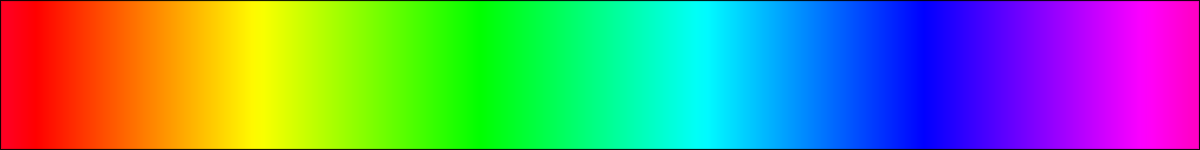
\includegraphics[width = 4.25cm, height = .3cm]{\here/colorbars/rb.png}};


\node[draw = black, thick, inner sep = 0pt, anchor = north] (cb4) at (group1 c2r1.south){
\includegraphics[width = 4.25cm, height = .3cm]{\here/colorbars/cividis.png}};
\node[draw = black, thick, inner sep = 0pt, anchor = north] (cb5) at (cb4.south){
\includegraphics[width = 4.25cm, height = .3cm]{\here/colorbars/batlow.png}};
\node[draw = black, thick, inner sep = 0pt, anchor = north] (cb6) at (cb5.south){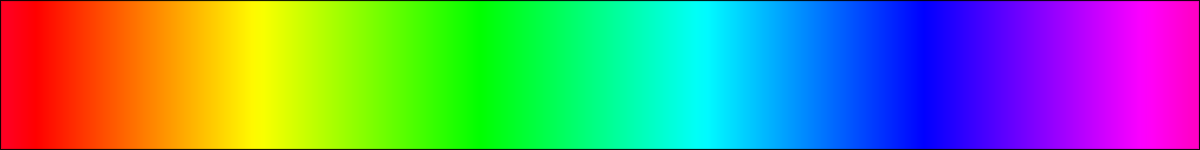
\includegraphics[width = 4.25cm, height = .3cm]{\here/colorbars/rb.png}};


\node[draw = black, thick, inner sep = 0pt, anchor = north] (cb7) at (group1 c3r1.south){
\includegraphics[width = 4.25cm, height = .3cm]{\here/colorbars/cividis.png}};
\node[draw = black, thick, inner sep = 0pt, anchor = north] (cb8) at (cb7.south){
\includegraphics[width = 4.25cm, height = .3cm]{\here/colorbars/batlow.png}};
\node[draw = black, thick, inner sep = 0pt, anchor = north] (cb9) at (cb8.south){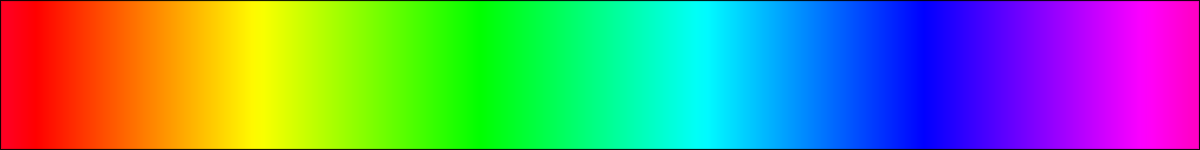
\includegraphics[width = 4.25cm, height = .3cm]{\here/colorbars/rb.png}};

\begin{groupplot}[
		group style = {
			group size = 3 by 1,
			vertical sep = .25cm,
			horizontal sep = .1cm, 
			},
		width = 4.25cm,
		height = 4cm,
		enlargelimits = 0.05,
		simpleax1,
		% ytick = {0,50},
		xticklabel = \empty,
		% xmin = 0.5,
		% xmax = 10.5,
		ymin = 0,
		ymax = 5.5,
		ytick pos = right, 
		yticklabel pos = right,
		scale only axis,
		enlargelimits = false,
		% xtick = {1.5,...,10.5},
		legend style = {
			at = {(0.5,1)},
			anchor = south,
			legend1},
		legend columns = 3,
		xtick = \empty,
		]


		\nextgroupplot[ymax = 100, ylabel = \empty, yticklabel = \empty]
		\addplot[ultra thick, hcqred]table[]{cmap_analytics/rb_L.txt};

		\nextgroupplot[xshift = .9cm, ylabel = \empty, yticklabel = \empty]
		\addplot[ultra thick, hcqred]table[y index = 1]{cmap_analytics/rb_d.txt};
		
		% \addlegendentry{$\Delta E^*_{ab}$}
		% \addlegendentry{$\Delta E^*_{2000}$}
		% \addlegendimage{hcqblue, ultra thick, mark = triangle*, mark options = {thin, fill = hcqblue, draw = black}};
		% \addlegendentry{$L$};
		

		\nextgroupplot[ylabel = \empty, yticklabel = \empty, ymax = 100, ytick pos = right, yticklabel pos = right]
		\addplot[hcqred, ultra thick]table[]{cmap_analytics/rb_d_cum.txt};
		% \addplot+[hcqred, ultra thick, mark options = {thin, fill = hcqred, draw = black}]table[y index = 2]{coldiff2000.txt};

		% \addlegendentry{$\Delta E^*_{ab}$}
		% \addlegendentry{$\Delta E^*_{2000}$}
		% \addlegendimage{hcqblue, ultra thick, mark = triangle*, mark options = {thin, fill = hcqblue, draw = black}};
		% \addlegendentry{$L$};


		% \nextgroupplot[]
		% \addplot+[hcqyellow, ultra thick, mark options = {thin, fill = hcqyellow, draw = black}]table[y index = 3]{coldiffLab.txt};
		% \addplot+[hcqred, ultra thick, mark options = {thin, fill = hcqred, draw = black}]table[y index = 3]{coldiff2000.txt};


		% \addlegendentry{$\Delta E^*_{ab}$}
		% \addlegendentry{$\Delta E^*_{2000}$}
		% \addlegendimage{hcqblue, ultra thick, mark = triangle*, mark options = {thin, fill = hcqblue, draw = black}};
		% \addlegendentry{$L$};

	\end{groupplot}

	\node[text width=1em, anchor=west]at(group1 c1r1.north west){\subcaptionbox{\label{cmA}}{}};
	\node[text width=1em, anchor=west]at(group1 c2r1.north west){\subcaptionbox{\label{cmB}}{}};
	\node[text width=1em, anchor=west]at(group1 c3r1.north west){\subcaptionbox{\label{cmC}}{}};
\end{tikzpicture}

	\caption{\textbf{Quantitative analysis of the three colormaps used in \figref{fig:sensitivityCVD}}. (a) Evolution of the lightness $L$ across the colormaps. (b) Distance between adjacent colors measured using the $\Delta E^*_{00}$ metric. Note that the absolut values for the different colormaps are not directly comparable. (c) Cumulative color distance from the starting color. A steady increase, as seen roughly in the scientific colormaps, ensures proportional mapping between numerical differences and perceptual changes. For more details, see the main text.}
	\label{fig:cmapanalytics}
\end{figure}



